\documentclass[12pt]{article}

%% Language and font encodings
%\usepackage[english]{babel}
%\usepackage[utf8x]{inputenc}
%\usepackage[T1]{fontenc}
\usepackage[margin=1in]{geometry}

%% Sets page size and margins
%\usepackage[a4paper,top=3cm,bottom=2cm,left=3cm,right=3cm,marginparwidth=1.75cm]{geometry}

%% Useful packages
\usepackage{amsmath}
\usepackage{graphicx}
%\usepackage[colorinlistoftodos]{todonotes}
%\usepackage[colorlinks=true, allcolors=blue]{hyperref}

\usepackage{caption, subcaption, xcolor}

\graphicspath{{res/}}

\title{Lab 2}
\author{Lukas Finkbeiner}

\begin{document}

\maketitle

\begin{abstract}

\textcolor{red}{We need more narrative drive. Consider using powerful transition phrases}

We investigated the hyperfine hydrogen transition by calibrating our measurements to thermal noise and by averaging over many blocks of data taken in optimal time windows of the day. We investigated the speed of light using waveguides (\textcolor{red}{How do they work?}). Our Chi-Squared analysis is completely deficient because our data were taken too broadly to show noticeable inconsistencies.

This is a great place to have a to-do section, because I prefer to write abstracts at the end of the writing process.

\quad * Ask Professor about the permissions thing (page 3), to make sure there are no technical difficulties.

\textcolor{red}{Figure out how to make the section headers smaller. They are taking up far too much space.}

\end{abstract}

% No need to re-derive anything!!

\section{Introduction and Background}

\textcolor{red}{Block diagram of the telescope electronics}. Fortunately, it seems like the professor took care of most of this for you in lecture, February 11.

% Leave the waveguide equations for the `models' section

% 3. The equations for the two waveguides; scipy.optimize.fmin

The data that we sample from the Big Horn via the PicoScope will feature arbitrary units which depend on our setup. To calibrate the intensity of the spectrum, we first calculate the gain:

\begin{equation}
G = \frac{T_\text{sys, cal} - T_\text{sys, cold}}{\sum (s_\text{cal} - s_\text{cold})} \sum s_\text{cold} \approx \frac{\text{300 K}}{\sum (s_\text{cal} - s_\text{cold})} \sum s_\text{cold}
\end{equation}

Where $T_\text{sys, cal} \approx 98.6^\circ$ F $\approx 310$ K represents the temperature of the human flesh that we use to cover most of the telescope. $T_\text{sys, cold}$ represents the temperature of the cold sky. We expect $T_\text{sys, cold} \ll T_\text{sys, cal}$, whereby we get the approximated form on the right. $s_\text{cal}$ represents the spectrum for which we attempt to maximize thermal noise in the collector, and $s_\text{cold}$ represents the spectrum for which we attempt to minimize.

To remove constant sources of interference in our data, we take an `on-spectrum' where 
Line shape:

\begin{equation}
s_\text{line} = \frac{s_\text{on}}{s_\text{off}}
\end{equation}

Putting it all together:

\begin{equation}
T_\text{line} = s_{line} \times G
\end{equation}

For our first experiment with waveguides, we seek to calculate to calculate the wavelength $\lambda_\text{sl}$ of a signal inside the waveguide based on the positions of the minima in the squared voltage, which we call nulls. We use the following equation for this first experiment; we expect a linear dependence of null spacings on $\lambda_\text{sl}$.

To plot our calibrated spectrum against Doppler velocity, we use the following relation:
\begin{equation}
v = -c \frac{\Delta \nu}{\nu_0}
\end{equation}

\begin{equation}
x_m = A + m \frac{\lambda_\text{sl}}{2}
\end{equation}

$m$ is the index of the null, $x_m$ is the position of the null $m$, and $A$ represents a constant offset which can represent whether the far end of the waveguide is open or shorted.

X-band waveguide \textcolor{red}{(this one requires more motivation):}

\begin{equation} \label{eq:xband}
\lambda_g = \frac{\lambda_\text{fs}}{[1 - (\frac{\lambda_\text{fs}}{2a})^2]^{1/2}}
\end{equation}

$\lambda_g$ is the guide wavelength, which we directly measure. $\lambda_\text{fs}$ is the free-space wavelength of the signal, which we will calculate using the known input frequency and the relation $c = f \lambda_\text{fs}$. $a$ is the width of the waveguide.

Here we define reduced chi-squared as follows:

\begin{equation}
\chi_r^2 = \frac{1}{N - M} \sum_i \frac{|y_i - \hat{y_i}|^2}{\sigma_i^2}
\end{equation}

\section{Methods}

% We used local oscillators at these power levels and at these frequencies.

To place our test signal in the upper and lower sidebands, we use these two frequencies. To put the hydgrogen in the upper and lower sidebands, we set the first local oscillator to these other two frequencies.

We measure $\lambda_g$, the guide wavelength, as the distance between the nulls in the guide output. We measure $a$ with a set of calipers and compare this with our results from a least-squares fit to the data based on equation \ref{eq:xband}.

% For the cass. data, we switched the local oscillator powers

\section{Observations}

As a preface, I may want to include commentary on how I had to manually alter the data, based on readings from the oscilloscope, in order to account for the imbalance in picoscope inputs?? I think not!

% The times of observation and why that matters.

% 1. initial calibration results. Here is a test signal. ``Our setup works!''
% source of error: angles are not aligned well. 10% error becomes... 25%? in power plot. I do not remember.

% scrap for time: justify the use of mean vs median

% talk about changes in the power levels for the local oscillators

% 2. initial H1 observations: on-line and off-line, to get the line shape
% difference between mean and median

% scrap for time: it doesn't look like our Cass data actually need a polyfit. We can probably
% just assume that it's flat already

\begin{figure}
\centering
\begin{minipage}{.45\textwidth}
	\centering
	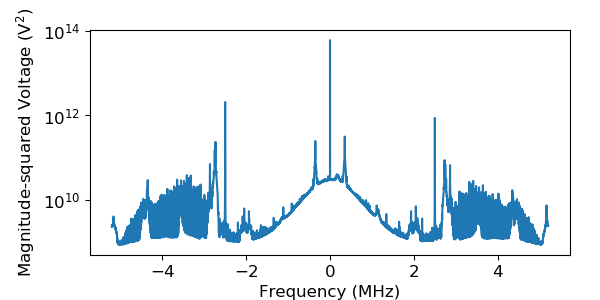
\includegraphics[width=\linewidth]{limits_justification}
	\captionof{figure}{A semi-log plot over the range of frequencies sampled. We assume that our 2 MHz low-pass filter works, so we will dismiss the signals farther than 2 MHz from the center. Additionally, the large central spike and smaller `bunny ear' spikes ($\pm$.5 MHz) appear on all data sets as persistent interference; we partially ignore these by limiting the y-axis. \textcolor{red}{Maybe you should use an initial test sample, to discuss this.}}
	\label{fig:on_limits}
\end{minipage} \hfill%
\begin{minipage}{.45\textwidth}
	\centering
	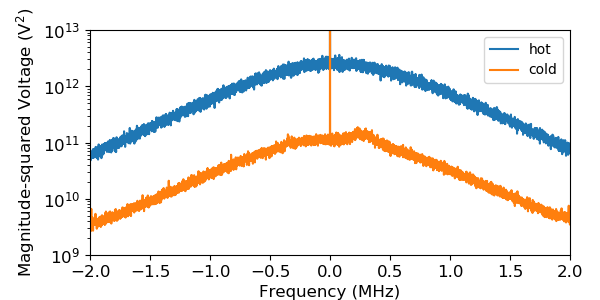
\includegraphics[width=\linewidth]{thermal}
	\captionof{figure}{The `hot' data correspond to three humans standing in front of the collector. The `cold' data correspond to the collector pointing up at the cold sky. The noise is not an issue because of its regularity: observe the even discrepancy between the curves over the domain of interest.}
	\label{fig:thermal}
\end{minipage}
\end{figure}

Figure \ref{fig:on_limits} shows a host of interfering signals, a consequence of the imperfections in our setup (such as low signal-to-noise ratio from low power on the local oscillators). \textcolor{red}{How can I justify ignoring the 2 MHz spikes? Aren't those bad?}

\begin{figure}
\centering
\begin{minipage}{.45\textwidth}
	\centering
	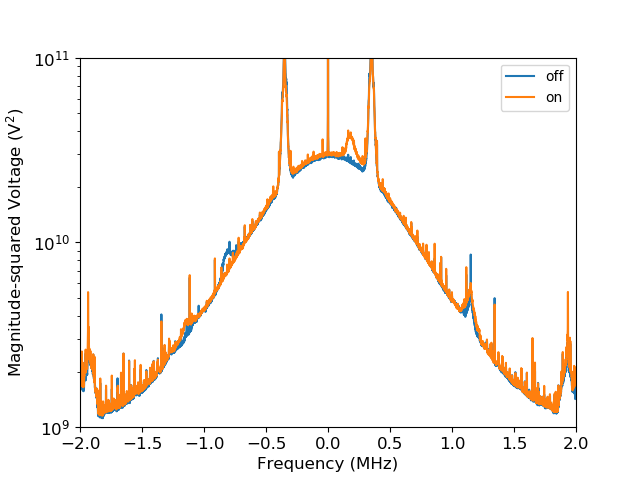
\includegraphics[width=\linewidth]{up_on_off}
	\caption{Combined plot of the `on' and `off' (LO1 at 1230 and 1231 MHz, respectively) power spectra. As we expect, the HI signal shifts by about 1 MHz between the two plots. This also supports our interpretation of the other patterns as interference: these patterns do not move between spectra.}
	\label{fig:up_on_off}
\end{minipage} \hfill%
\begin{minipage}{.45\textwidth}
	\centering
	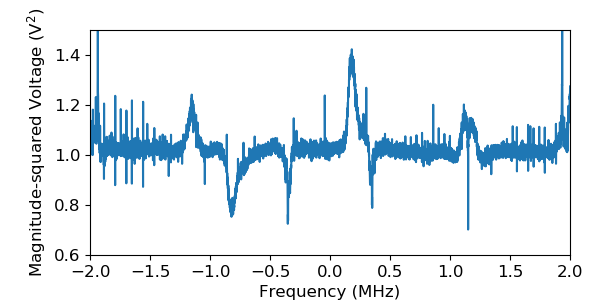
\includegraphics[width=\linewidth]{up_shape}
	\caption{\textcolor{red}{This one is not helpful. Replace it with the final, calibrated spectrum, thermal power units.}}
	\label{fig:up_shape}
\end{minipage}
\end{figure}

\textcolor{red}{These data were recorded between x and y, which corresponds to, via the rotation matrices}. Since the Horn was pointing straight up, we may say that the declination is equal to the latitude of the telescope. In our case, that is $37.873188^\circ \approx 0.661012$ radians.

The right ascension is equal to the local sidereal time (LST) of data-capture. We began our data capture at 1582937209.9447305 seconds after 1970 and completed our data capture at 1582937704.4486437 seconds after 1970.

We took all of our data in unix time. Here is the conversion table.

\textcolor{red}{I forgot when we did the cold sky data}

Included below is a table including examples of date conversions for the events of interest to Doppler corrections. \textcolor{red}{When converting from galactic to $equatorial$, we do not need to take into account the time at which we measured}. Therefore, we omit those data from the table. %For the sake of brevity, we omit the counterparts for the Cassiopeia measurements.

\

\begin{center}
 \begin{tabular}{||c c c||} 
 \hline
 Label & Unix Time & Julian Date \\ [0.5ex] 
 \hline\hline
 On-line start & 1582937209.9447305 & 2458908.5325225084 \\ 
 \hline
 On-line stop & 1582937704.4486437 & 2458908.5382459336 \\
 \hline
 Off-line start & 1582937837.5090616 & 2458908.5397859844 \\
 \hline
 Off-line stop & 1582938387.1761112 & 2458908.5461478718 \\ [1ex] 
 \hline
\end{tabular}
\end{center}

\begin{center}
 \begin{tabular}{||c c c||} 
 \hline
 Label & LST & PST\\ [0.5ex] 
 \hline\hline
 On-line start & 0.8334479646673989 & 2/28/20 @ 16:46:49 \\ 
 \hline
 On-line stop & 0.8695077621535888 & 2/28/20 @ 16:55:04 \\
 \hline
 Off-line start & 0.8792106794915676 & 2/28/20 @ 16:57:17 \\
 \hline
 Off-line stop & 0.9192930359644231 & 2/28/20 @ 17:06:27 \\ [1ex] 
 \hline
\end{tabular}
\end{center}

\

% 4. Plot waveguide results, at least for the xband, to talk about how weird everything is.
% caliper measurement for a. 'This is what we hope to get from analysis'
% sources of error.

\section{Analysis}

% 1. The poly fit to the baseline

% 2. The Gaussian fits to the remaining curves

% 3. 

\section{Conclusions}


\section{Acknowledgments}

\textcolor{red}{You have to remedy your complete ignorance of BibTex}

\end{document}
